%% ============================================================
%%  Figura: flujo de cribado PRISMA 2020.
%%  Cifras tomadas de "Protocolo PRISMA/Bitacora_revision_sistematica.docx"
%%  (etapas 4 y 5): 319 identificados, deduplicacion -98, filtro DOI -20,
%%  filtro de accesibilidad -64, corpus final de 25 en
%%  "Referencias_seminario.xlsx". No se toma ninguna cifra del corpus
%%  obsoleto de "Analisis 137 referencias.xlsx".
%%
%%  Se compila POR SEPARADO y se incluye como PDF con \includegraphics,
%%  porque main.tex no se toca (regla de aislamiento de CLAUDE.md).
%%
%%  Regenerar con:  pdflatex -interaction=nonstopmode prisma_flujo.tex
%% ============================================================
\documentclass[border=2pt]{standalone}
\usepackage[T1]{fontenc}
\usepackage[utf8]{inputenc}
\usepackage{times}
\usepackage{tikz}
\usetikzlibrary{arrows.meta, positioning}

\definecolor{bordeCaja}{gray}{0.35}
\definecolor{fondoCaja}{gray}{0.95}

\begin{document}
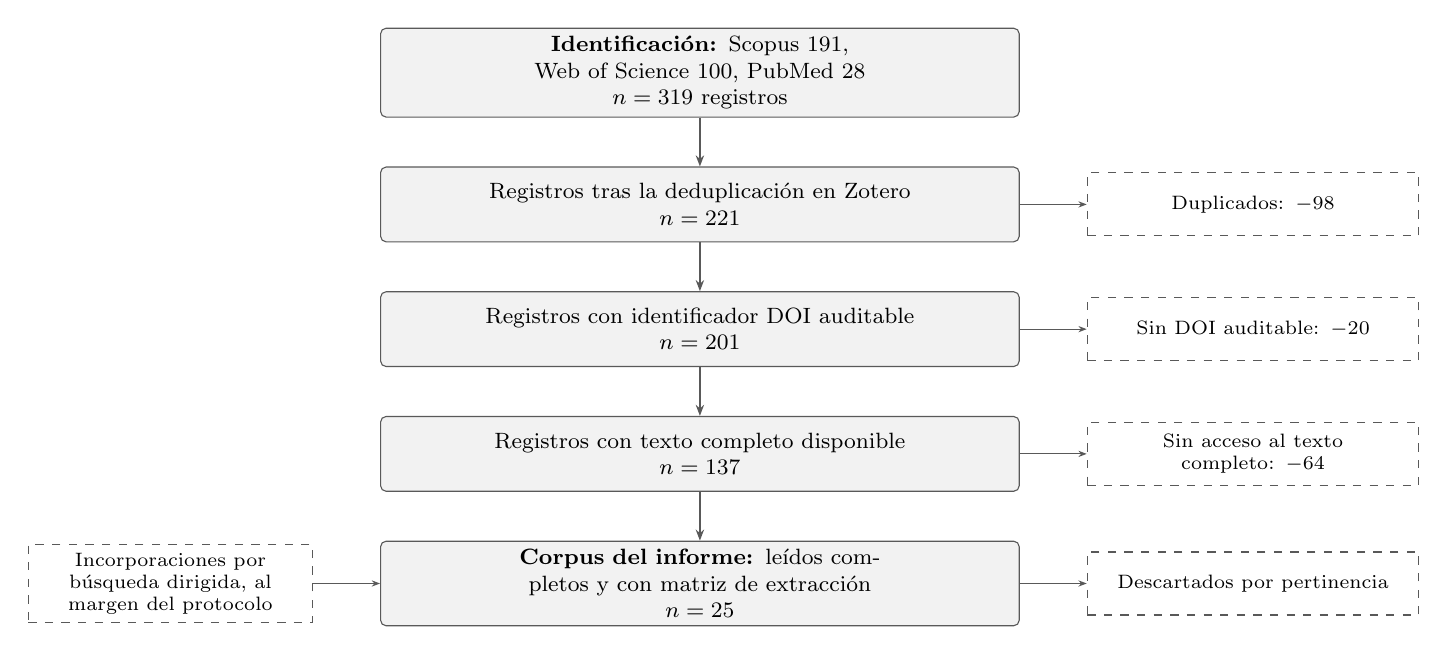
\begin{tikzpicture}[
  font=\footnotesize,
  paso/.style={draw=bordeCaja, fill=fondoCaja, rounded corners=2pt,
               text width=7.9cm, minimum height=0.95cm,
               align=center, inner sep=3pt},
  salida/.style={draw=bordeCaja, dashed, text width=4.0cm,
                 minimum height=0.8cm, align=center, inner sep=3pt,
                 font=\scriptsize},
  entrada/.style={draw=bordeCaja, dashed, text width=3.4cm,
                  minimum height=0.8cm, align=center, inner sep=3pt,
                  font=\scriptsize},
  flecha/.style={-{Stealth[length=4pt]}, draw=bordeCaja, thick},
  lateral/.style={-{Stealth[length=3pt]}, draw=bordeCaja}
]

\node[paso] (id) {\textbf{Identificación:} Scopus 191, Web of Science 100, PubMed 28\\ \mbox{$n = 319$ registros}};
\node[paso, below=0.62cm of id] (dedup) {Registros tras la deduplicación en Zotero\\ \mbox{$n = 221$}};
\node[paso, below=0.62cm of dedup] (doi) {Registros con identificador DOI auditable\\ \mbox{$n = 201$}};
\node[paso, below=0.62cm of doi] (texto) {Registros con texto completo disponible\\ \mbox{$n = 137$}};
\node[paso, below=0.62cm of texto] (final) {\textbf{Corpus del informe:} leídos completos y con matriz de extracción\\ \mbox{$n = 25$}};

\draw[flecha] (id) -- (dedup);
\draw[flecha] (dedup) -- (doi);
\draw[flecha] (doi) -- (texto);
\draw[flecha] (texto) -- (final);

\node[salida, right=0.85cm of dedup] (s1) {Duplicados: \mbox{$-98$}};
\node[salida, right=0.85cm of doi] (s2) {Sin DOI auditable: \mbox{$-20$}};
\node[salida, right=0.85cm of texto] (s3) {Sin acceso al texto completo: \mbox{$-64$}};
\node[salida, right=0.85cm of final] (s4) {Descartados por pertinencia};

\draw[lateral] (dedup) -- (s1);
\draw[lateral] (doi) -- (s2);
\draw[lateral] (texto) -- (s3);
\draw[lateral] (final) -- (s4);

\node[entrada, left=0.85cm of final] (extra) {Incorporaciones por búsqueda dirigida, al margen del protocolo};
\draw[lateral] (extra) -- (final);

\end{tikzpicture}
\end{document}
